\documentclass[11pt,a4paper]{article}
\usepackage{hyperref}
\usepackage{fancyhdr}
\usepackage{fancybox}
\usepackage{multirow}  
\usepackage{times}
\usepackage{cite}
\usepackage{graphicx}
\usepackage{graphics}
\usepackage{amsfonts}
\usepackage{amssymb}
\usepackage[left=1.25in,right=1in,top=1in,bottom=1in]{geometry}
\usepackage{float}
\usepackage[latin2]{inputenc}
\usepackage{ulem}
\usepackage{inputenc}

\begin{document}
%------------------------------ Start of Front Page------------------------------------
\newpage
\pagestyle{empty}
 \pagenumbering{gobble}
 
\begin{center}
\textbf{\Large{A Project Based Seminar Report}}
\end{center}

\begin{center}\textbf{on}
\end{center}
			
\begin{center}
\textbf{ \Large{\textbf{ \lq \lq The Cyberspace: Redefining A New World \rq \rq}}}
\end{center}
     
\begin{center}Submitted to the 
\end{center}

\begin{center}\large{Savitribai Phule Pune University}
\end{center}

\begin{center}In partial fulfillment for the award of the Degree of
\end{center}

\begin{center}\large{Bachelor of Engineering} 
\end{center}

\begin{center}in
\end{center}

\begin{center}\large{Information Technology}
\end{center}

\begin{center}by
\end{center}

\begin{center}
\textbf{\Large{ \textbf{Priyatosh Kadam}}}
\end{center}

\begin{center}\textbf{(Exam Seat No.)}
\end{center}

\begin{center}Under the guidance of
\end{center}

\begin{center}\textbf{\Large{\textbf{R. M. Kawale}}}
\end{center}

\begin{center}
\begin{figure}[h]
			\centering
			\includegraphics[width=2.5 cm]{COEMlogo}
\end{figure}
\end{center}
	
\begin{center}Department of Information Technology
\end{center}

\begin{center} \large {PDEA's College of Engineering, Manjari (Bk.)}
\end{center}

\begin{center}Pune - 412307.\textbf{ }
\end{center}


\begin{center}\textbf{\large{2022-2023}}
\end{center}
%------------------------------------- End of Front Page------------------------------------
%-------------------------------- Start of Certificate Page----------------------------------
\newpage
\pagestyle{empty}
\pagenumbering{gobble}

\begin{figure}[h]
\centering

\includegraphics[width=4cm,height=4cm]{COEMLogo.jpg}
\end{figure}

\begin{center}
\textbf{\Large{CERTIFICATE}}
\end{center}

\textsf{This is to certify that the project based seminar report entitled \textbf{\lq \lq Title of seminar\rq \rq} being submitted by \textbf{XYZ (Exam Seat No.)} is a record of bonafide work carried out by him/her under the supervision and guidance of \textbf{Prof. R. M. Kawale} in partial fulfillment of the requirement for \textbf{TE (Information Technology)-2015  Course} of Savitribai Phule Pune University, Pune in the academic year 2018-2019.}

\begin{quote}
Date:\textbf{30/03/2018}\\
Place:Manjari (Bk.), Pune
\end{quote}

\vspace{0.2 in}

\begin{center}
\textbf{Prof. R. M. Kawale} \hspace{150pt} \textbf{Prof. N. R. Jain}\\
\hspace{62pt}{Guide} \hspace{165pt} Head of the Department
\end{center}

\begin{center}\textbf{Dr. R. V. Patil}\\ 
{Principal}
\end{center}

\par\noindent\rule{\textwidth}{0.4pt}
This Project Based Seminar report has been examined by us as per the Savitribai Phule Pune University, Pune requirements at PDEA's College of Engineering, Manjari (Bk.), Pune - 412 307  on . . . . . . . . . . .
\\
\begin{center}
Internal Examiner  \hspace{200pt}External Examiner
\end{center}

%-------------------------------- End of Certificate Page----------------------------------
%------------------------------Start of Acnowlegement Page----------------------------------
\newpage
\pagestyle{empty}           
\pagenumbering{roman}

\begin{center}\textbf{\Large{ACKNOWLEDGEMENT}}
\end{center}
In completing this project report study on project titled The Cyberspace: Redefining A New World , I had to 
take the help and guideline of a few respected people, who deserve my greatest gratitude. 
The completion of this project report gives me much Pleasure. I would like to show 
my gratitude to Prof. R.M.Kawale for giving me a good guideline for project throughout 
numerous consultations. I would also like to expand my deepest gratitude to all those who
have directly and indirectly guided us in writing this project report. 
Many people, especially my classmates and friends themselves, have made valuable 
comments and suggestions on this proposal which gave me inspiration to improve my project. 
Here I thank all the people for their help directly and indirectly to complete this project
report.




\vspace{0.5 in}

(Students Name \& Signature) 
%-------------------------------- End of Acnowlegement Page----------------------------------
%----------------------------------Start of Abstract Page-----------------------------------
\newpage

\begin{center}\textbf{\large {Abstract}}
\end{center}

Most difficult and important component of report/seminar is to write abstract. Presented at the beginning of the report, it is likely the first substantive description of your work read by an external examiner/reader. You should view it as an opportunity to set accurate expectations. The abstract is a summary of the whole project work.\\ 

It presents all the major elements of your work in a highly condensed form. An abstract often functions, together with the project title, as a stand-alone text. An abstract is not merely an introduction in the sense of a preface, preamble, or advance organizer that prepares the reader for the report.\\

In addition to that function, it must be capable of substituting for the whole report when there is insufficient time and space for the full text. The final version of the abstract will need to be written after you have finished reading your report for the last time. However, if you think about what it has to contain, you realize that the abstract is really a summary of your project/seminar work.\\

Your abstract should answer specifi questions: What was done? Why was it done? How was it done? What was found? What is the signficance of the findings?

%-------------------------------- End of Abstract Page-----------------------------------------
%----------------------------Start of Content and other  Pages---------------------------------
\newpage

\begin{normalsize}
\pagestyle{empty}
\pagenumbering{roman}	

\begin{center}
			
\tableofcontents
\end{center}					

			     
			         
\newpage
\pagestyle{empty}
\pagenumbering{roman}

\begin{center}
{
\setlength{\baselineskip}{1.5\baselineskip}\listoffigures\addcontentsline{toc}{section}{List of Figures}
}
\end{center}

			         
\newpage
\pagestyle{empty}
\pagenumbering{roman}	

\begin{center}
{\setlength{\baselineskip}{1.5\baselineskip}\listoftables\addcontentsline{toc}{section}{List of Tables}
}
\end{center}	          
\end{normalsize}
%---------------------------- End of Content and other  Pages---------------------------------
%---------------------------- Start of Header and Footer  Page---------------------------------
\newpage
\pagestyle{fancy}
\pagenumbering{arabic}

\fancyhead[RO]{\textit{Title of Seminar}}                                                 % Right over part of header
\fancyhead[LO]{\textit{Project Based Seminar}}			 % Left over part of header
\renewcommand{\footrulewidth}{0.5pt}	     			 % command to change footer ruler width
\fancyfoot[RO]{\textit{PDEA's COE, Manjari (Bk.), Pune}} % Right over part of footer
\fancyfoot[LO]{\textit{Dept. of Info. Tech. 2018-19}}	 % Left over part of footer
%---------------------------- End of Header and Footer  Page---------------------------------
%---------------------------- Start of First Chapter---------------------------------
\newpage
\begin{center}
\section{INTRODUCTION TO PROJECT TOPIC}
{\setlength{\baselineskip}{1.5\baselineskip} }									
\end{center}

\subsection{ Introduction to Project Topic}

\par Students are expected to write brief introduction of the project topic. This section may be common for all the students of that group. However students can have different approach in explaining their project.
\\

Since we are not going to get separate project report from the students, 
it is good to have one or two pages common for all the students of that 
project. Once this project introduction and aim objectives of explained, 
students can start with actual seminar content writing.

\subsection{ Motivation behind project topic}

Students are expected to write "\,Why they thought about this project". 
They could also explain the "\,Explain need of the project". Any 
statement which motivated to take up this project

\subsection{ Aim and Objective(s) of the work}

\textbf{Project aims} are a statement of the overall "\,Why" of the 
project. A project aim is a statement starting with the words: "\,The 
aim of this project is\ldots "
\\

That statement tells the reader what your overall goal is, what it is 
you want to achieve. It does not go into details or describe specific 
tasks.
\\

\textbf{Project objectives} tell the "\,How" of the project aim. You 
want to achieve your goal and the objectives state how this will be done 
- what major tasks will be undertaken and what your major targets 
are. Most projects will have between six and nine objectives. A project 
objective is usually a statement starting with the words "\,To\ldots " 
\\

Objectives are subsidiary to aims and are the steps you are going to 
take to answer your problem statement or a specific list of tasks needed 
to accomplish the goals of the project. This must be highly focused and 
feasible and should address the more immediate project outcomes
\\
Guide must personnel check these aim and objectives and make students 
write these statements properly.

\subsection{ Introduction to Seminar Topic}

Internal guides need to clearly identify separate topics for individual 
students while preparing seminars. It should be based on project topic/area.
\subsubsection{Aim and Objectives of Seminar}

\begin{itemize}
\item {\textbf{Aim}}
\paragraph{}Write here AIM of Seminar.\\
\item {\textbf{Objectives}}
\paragraph{}Write here Objectives of Seminar.
\begin{enumerate}
\item Objective 1. 
\item Objective 2. 
\item Objective 3.
\item Objective 4 and So on.
\end{enumerate}
\end{itemize}

\subsection{ Organization of the Report}



%---------------------------- End of First Chapter------------------------------------
%---------------------------- Start of Second Chapter---------------------------------
\newpage
\begin{center}
\section{LITERATURE SURVEY OF Seminar Title/Topic}
{\setlength{\baselineskip}{1.5\baselineskip} }									
\end{center}

Students are expected to write similar or related work already done by various researchers. They could also explain existing tools/technologies in this section. There advantages and disadvantages of each method or technique. They should also explain how their project is different from those existing systems. You need to read lot of books/ papers/ magazines for making this survey.

\begin{figure}[h]
\centering
 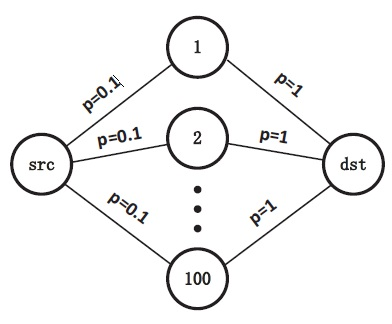
\includegraphics[]{1}
\caption{Example Diagram}
\end{figure}
\newpage
\begin{center}
\begin{table}
\caption{Tabe no.3.2 Vulnerabilities, Threats & Risks }\\

\begin{tabular}{|p{8cm}|l|l|l|}
\hline 
\centering\textbf{Incidents} & \textbf{Jan-June 2012} & \centering \textbf{Jan-June 2013 } & \textbf{ Increase/ (decrease)}  \\ 
\hline 
Fraud & 2439 & \centering{2490} & 2   \\
\hline 
Intrusion & 2203 & 1726 & 22  \\
\hline
Spam & 291 & 614 & 111  \\
\hline
Malicious code & 353 & 442 & 25   \\
\hline
Cyber Harassment & 173 & 233 & 35  \\
\hline
Content related & 10 & 42 & 320    \\
\hline
Intrusuion Attempts & 55 & 24 & 56  \\
\hline
Denial of Services & 12 & 10 & 17  \\
\hline
Total & 5581 & 5592 &     \\
\hline
\end{tabular} 
\end{table}
\end{center}
%---------------------------- End of Second Chapter---------------------------------
%---------------------------- Start of Third Chapter---------------------------------
\newpage
\begin{center}
\section{SEMINAR RELATED OTHER CHAPTERS}
{\setlength{\baselineskip}{1.5\baselineskip} }									
\end{center}

\textbf{3.1   Cyberspace vs Internet }\\
\begin{center}


Internet is a network of networks, what that means is that it is a global network that is creating by linking smaller networks of computers and servers. Cyber-space is nothing more than a symbolic and figurative space that exists within the scope of Internet.
There is a lot of confusion between the usage of the terms, Cyberspace and Internet. Many people think that the words mean the space, while others think that they mean two completely different things within the field of technology. The truth of the matter is that it is something in the middle. The terms do mean two different things, but the confusion arises due to the fact that these things are closely interrelated, due of which they are often mistakenly used interchangeably.
The term cyberspace has led to the introduction of other words, such as cyber security, cyber-crime, cyber-war, cyber-terrorism, etc. Cyberspace itself comes from cybernetics, which in turn is derived from the Ancient Greek kybernetes, which means steersman, governor, pilot, or rudder.
The term cyberspace came into being in regard to managing physical spaces. However, with the onset of the Internet, the term has been applied to the virtual space that is created within the Internet.
Cyberspace is nothing more than a symbolic and figurative space that exists within the scope of Internet. It can be said that anything that is done via the use of Internet, occurs within the confines of the cyber-space, whether that is sending an e-mail, a website, or playing a game, all of these things exist within the cyber-space.
Internet, on the other hand, is a network of networks, what that means is that it is a global network that is creating by linking smaller networks of computers and servers. This network allows users to share information and other data from one point to another. The data can be in the form of text, image, or video.
The terms might be easier to explain the terms via the use of an example. Think of a book. The book itself is akin to the Internet. It is a way for the information, i.e. story or text, to be conveyed from the author to the reader, similar to how the Internet transfers data between two computers (or server and a computer).
Now the reader reads the story and imagines it in their mind as a virtual reality that is playing out the story via the characters and dialogues. This virtual reality is the cyberspace. It is how the reader or the user imagines the information that is transferred via the Internet/book.
\end{center}
\begin{center}
\begin{figure}[h]
			\centering
			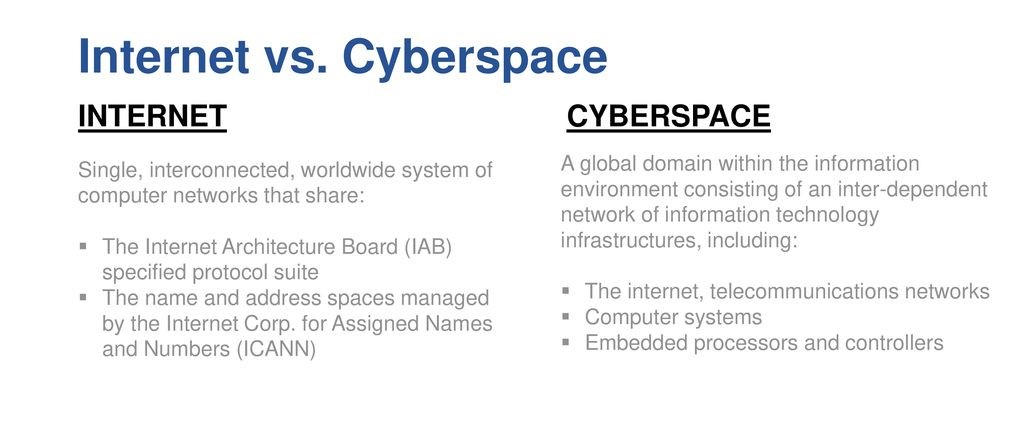
\includegraphics[width=15 cm, height =9 cm]{diff.jpg}
\end{figure}
\end{center}


\texbf{ 3.2.1 The Three Major Trends}

	The purpose of this section is to identify these evolutionary trends and to extrapolate their implications. This section focuses on the accumulation
of incremental evolutionary change over long periods.Even individually small quantitative changes, when compounded over time, can bring about great
qualitative changes on their own. In addition to evolutionary trends, revolutions are also possible.Trends that have transformative implications will be examined, while fads and flash in the pan issues will be ignored, even though it is not always easy to see the difference while in the midst of major transformations\\

\texbf{ 3.2.1 Computer and network trends }\\

	Among the computer and network trends likely to have lasting effect are: increases in computer and network power, proliferation of broadband and wireless
connectivity, and upgrades in the fundamental protocols of the Internet.
Increase in computer and network power\\
 
\texbf{Broadband proliferation}\\
	Another major evolutionary trend in cyberspace is the widespread deployment of broadband Internet services. Cyberspace experienced at a speed of just 56 kilobytes per second, allowing rudimentary Web surfing and data exchange—is very different from cyberspace at 400 kbps or more. Widespread access to faster connectivity by desktops, laptops, personal digital assistants, and cell phones enables new business models and new social interactions. Just as business and social models were transformed by the move from trains and ocean liners to jet airline flights in the past century, today the richer audio, video, and networked
applications supported by higher speed Internet connections make cyberspace significantly more valuable to its users. Many face-to-face transactions and
physical exchanges can be supplanted by much less expensive software-based interactions. New services not previously associated with the Internet, including
telephony and television, are moving to this plentiful cheap bandwidth. Widespread fiber optics, cable modems, digital subscriber loops/lines (DSL), and
broadband wireless services are the technological underpinnings allowing broadband access by consumers or businesses throughout the world (ITU.2004). These technologies have higher speeds(typically greater than 400 kbps) and are also always on, not requiring time consuming dial up handshakes. While broadband deployment is already a reality in many parts of the world, it is not yet universal. Some set of users probably will continue to use dial-up access
for some time, but there are likely to be fewer and fewer. Broadband connectivity to the endpoints of computer communication is only possible if the Internet
backbone itself can carry all of the extra traffic generated by these end systems. Internet backbone providers have deployed more high-speed links, using
new fiber technologies such as OC–48 and OC– 192 with operating speeds of 2.488 Gigabits per second and 10 Gigabits per second, respectively. Higher speed satellite and microwave towers are interconnecting high-speed networks around the
world. Interconnectivity between various backbone providers has increased to carry more traffic more quickly. As this interconnectivity grows, the topology
of the Internet backbone becomes more complex from a design and management perspective. As client computers increasingly rely on broadband access, and
as the Internet infrastructure is refined to carry all of those bits, the servers to which the communications are directed likewise need additional computational and network power to provide new services. Faster servers
can help deal with some of these needs, but most large Internet companies are instead relying on larger numbers of less expensive servers, distributed across
one or more campuses around the world. Large Internet companies (Google, Amazon, eBay, and Microsoft) are constructing vast server farms. For instance, Google‘s
server count was half a million computers in 2007. Business models are also evolving, as Internet service providers (ISPs) try to furnish value-added
services and applications on top of their increasingly commoditized bandwidth business. To realize the business value in the telephony, video, and various
other applications and content being distributed via their pipes, some ISPs are partnering with, buying, or building in-house application services and content.
Such services and content are directly affiliated with that ISP, in contrast to other services that are not affiliated but that are accessed through that ISP by its customers. This evolution has led some ISPs to consider
charging non affiliated application service providers and users a premium for their use of high bandwidth. Those that do not pay extra may face lower
performance, with their traffic handled at a lower priority than higher paying affiliated users and
application providers. This economic friction between ISPs and
application service providers is a worldwide
phenomenon and has been termed the Net neutrality issue. Some argue that governments should require the equal or neutral handling of affiliate and non-affiliate traffic alike by ISPs, to foster interoperability and prevent the fragmentation of the Internet into various ISP enclaves\\

Wireless proliferation \\

Cyberspace connectivity is increasingly moving to wireless communication, in the form of wireless local area networks (WLANs), wireless broadband, and similar technologies. One of the major vectors of this move is often overlooked in discussions of cyberspace the cell phone. An estimated two billion people have access to cell phones. Over 150 million camera phones have been sold to date, each supporting voice, text, and image transfer. Even with low
bandwidth text messaging, their small size, decentralized communications capacity and relatively low cost have made cell phones an increasingly important technology underlying social change
	Where today‘s cell phones have simple text messaging and still cameras, future cell phones with higher bandwidth applications and full video
capabilities are likely to have even greater impact as they gain the capabilities of modern personal computers and become, in effect, pocket-sized television studios. The hand-held video cameras of the late 1980s and early 1990s led to countless major news stories, such as the 1992 Rodney King riots in Los Angeles. However, that technology was limited: few people carried
cameras with them most of the time, and the technology required the cumbersome handling of physical videotapes, typically delivered by hand or by courier.
By contrast, when a major portion of the world‘s population carries cell phone–based video cameras wirelessly linked to the Internet at all times,
cell phones will likely have a much larger impact on society, as when camera-equipped cell phones disseminated graphic pictures and video, albeit of low
quality, of the execution of Saddam Hussein in 2006 within minutes of the event. Today‘s grainy cell phone photos and simple videos will be replaced by much
better multi-megapixel video cameras integrated into cell phones as video capture technology becomes smaller, cheaper, and more widely disseminated. Already television news outlets in some countries ask members of the public to submit cell phone video of events immediately after they happen. Web sites offer
to broker the sale of videos of hot news events taken by private individuals. These trends decrease the time between an event‘s occurrence and its coverage in the news, further shrinking the news reporting cycle and the time available for the public and policymakers to analyze events.
 Numerous other wireless technologies are transforming the nature of cyberspace. WLANs, in their most popular form, are implemented according to a set
of standards denominated 802.11. Such WiFi networks allow nearby systems (within perhaps 100 meters) communicating with one another or gaining access to the Internet. Computers from wired access make it possible to use them for a wider variety of applications, ranging from industrial use to home
appliances. By minimizing the need for costly wiring installations, WLANs allow for more rapid network deployment at much lower costs. A variety of organizations have taken advantage of this\\

Transition from IPv4 to IPv6\\
 
The current Internet infrastructure is based on the widely deployed IPv4, a specification originally created in the late 1970s that spread widely in the early
1980s and throughout the 1990s as the Internet grew. This protocol far exceeded its original expectations,becoming the common language for communication
across the Internet and large numbers of private networks, and allowing a huge variety of devices—from mainframe systems to cell phones—to communicate.
Despite its unprecedented success as a protocol, the original IPv4 design had significant drawbacks: a limited number of network addresses that were
distributed inefficiently, no built-in support for security, a lack of quality-of-service features, and limited support
for mobile devices. To address these shortcomings, the Internet
Engineering Task Force set out in the mid-1990s to define a next-generation Internet protocol, termed IPv6. While the IPv6 specifications were completed sometime ago, full deployment has been slow. Most modern
operating systems have IPv6 software, but few use it.Pockets of IPv6 networks exist in specialized laboratory and educational environments. Small IPv6 networks
have been overlaid on the existing IPv4 Internet, with network nodes run by academics, researchers, and hobbyists around the world. One of the major reasons
IPv6 deployment has moved slowly involves the innovative retrofitting of its various concepts into the existing IPv4. (30) Most organizations have deployed
various network address translation devices to shuffle and reuse private network addresses, somewhat alleviating the original constraints of IPv4‘s 32-bit
addresses. Likewise, quality of service and mobility options have been implemented in IPv4. These adaptations to IPv4‘s limits have eased many of the pain points driving the demand for IPv6. Although IPv6 deployment has started slowly,
it is expected to ramp up; both the Chinese government and the U.S. military have announced intentions to move to IPv6 to support the modernization of their
large networks. Even so, some Internet experts have viewed IPv6 deployment as a perpetual five years in the future always predicted, but never actually
occurring. However, over the next decade, IPv6 deployment seems very likely, given the momentum of decisions by large buyers, large vendors, (30) and the
Internet Engineering Task Force, which crafts the specifications for the protocols used on the Internet.Building and maintaining IP stacks is very
difficult, even using the far simpler IPv4 protocol. The
software development community has required a full 20 years to scrub similar problems due to faulty code out of their IPv4 implementations.8 IPv6 software is likely to go through a similar process as vulnerabilities are discovered and fixed. While it may not take another 20 years to get IPv6 right, it will certainly require significant effort to discern flaws in the numerous implementations of this vastly more complex protocol. The Internet and its users may be exposed to attacks for some time. IPv6 also raises other security implications.
The very large address space can make it easier for systems to hide: an attacker who modulates a network address across a very large address space can hide
systems more easily than within the smaller and simpler IPv4 landscape.\\
\begin{center}
\begin{figure}[h]
			\centering
			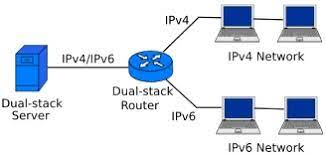
\includegraphics[width=10 cm]{ipv4.jpeg}
\end{figure}
\end{center}\\
\	3.2.1 Software trends\\
 	
 	Among the software trends likely to have
lasting effect are: increases in software complexity; enhanced capabilities for search both across local systems and Internet-wide; widespread virtualization of
operating systems convergence of technologies increased noise in most aspects of cyberspace increased vulnerability due to advancement of computer and network attack and exploit methodologies.\\

 Increases in software complexity\\
 
 	Although underlying hardware and network speeds have increased, most new computers do not seem to their users to be significantly faster than their
predecessors for very long after their introduction. This is largely due to increases in software complexity, as additional features, increased error-handling
capabilities, and more complex security facilities sap the processing gains reflected in MoorEs law and in higher bandwidth. Modern software includes a
proliferation of features, some important and useful to large numbers of users, and others providing utility to only a small fraction of the user base. Users demand that new programs do more than their old software, and
vendors cater to this expectation. Software vendors introduce these features to entice new customers to purchase their products, as well as to inspire existing
customers to continue on the treadmill of constant software upgrades. Unfortunately, some software vendors do not spend the resources necessary for
thorough development, integration, and testing of these features and modifications. More complex software is more likely to have
flaws, which may manifest themselves in broken features, software crashes, or security vulnerabilities. When a software flaw is discovered, especially one with
major security implications, the software vendor typically releases a patcH to alleviate the condition. Microsoft, for example, releases patches once per
month, each typically including between five and a dozen major fixes, often requiring upwards of 10 megabytes of new code. With such massive changes
pushed to over 100 million systems, the patching process for Windows alone is a monumental worldwide undertaking on a monthly basis, involving not just
Microsoft, but also hundreds of thousands of enterprise users and consumers, not all of whom test such patches carefully before installing.
Moreover, multiple patches applied over time could introduce additional flaws. The constan accumulation of patches can make systems more
brittle, requiring even more complexity to patch adequately without breaking functionality. Unfortunately, complexity is often the enemy of
security, as subtle vulnerabilities linger in highly complex, perhaps poorly understood code. To address such vulnerabilities, security tools—antivirus tools,
antispyware software, and intrusion prevention systems—are common defences for systems today. Many of these tools operate in a reactive fashion, to
clean up after an infection has occurred, and most defend against specific vulnerabilities that have already been found, not against as-yet-undiscovered security flaws. Compounding the problem, these security tools themselves often have flaws, so they need patches as well. This, again, increases the overall complexity of computer systems and makes them even more brittle.
Antivirus, antispyware, and other anti–malicious code technologies use a mixture of techniques to detect such malware,analyzing protected computers on which
they are installed at a granular level to police the system for infection and attacks. The need for such defence is turning into a significant security tax on the increases described by Moores law and is boosting complexity.\\

Enhanced search capabilities \\

	With increasingly complex software used for a
greater number of applications, more and more vital data is accumulating in databases and file systems. On a local system, data are typically stored in multi-Gigabyte or even Terabyte (1,000 Gigabyte) file systems. On large servers or even networked groups of systems, databases often exceed 100 Terabytes. These data are
only useful if users and applications can search for information; high-quality search functionality is therefore vital, and the data must be organized, stored,
and presented in useful structures. The metadata that describe the data, tagging, and visualization technologies are thus increasingly critical. Because of
their involvement with these crucial functions, Internet search engines are currently at the centre of activity in cyberspace evolution. As search engines acquire more data sources, including phone books, highly detailed
satellite imagery, and maps, users are presented with more powerful search directives and operators. Such options let users hone in on specific
items they seek, using a complex array of search directives instead of merely grabbing data with a specific set of search terms located in it. In addition,
simple text-based searches are expanding to searches for images, sound, or videos. With so much information on the Internet, many users need help to find what they
need. Users might not even know precisely what to search for and would benefit from a ranking system of interesting or useful sources of information. To address
this need, other sites on the Internet act as aggregating front-end portals that organize data from multiple data sources and process it to provide users with extra value. Sites such as digg.com and del.icio.us contain lists of
popular articles and sites that are voted on by users, giving other users a guide to information in a variety of categories The need for search capabilities is not limited to the Internet. Internal network searching is increasingly important for locating useful information from an organization‘s internal servers and desktop
computers.\\

Widespread operating system virtualization\\

	Virtual machine environments (VMEs) such as
VMware, Microsoft‘s Virtual Server, and Xen let a user or administrator run one or more guest operating systems on top of a single host operating system. With
such VME tools, for example, three or four instances of the Microsoft Windows operating system can run as guest systems on top of a single Linux host operating
system on a single PC or server. The concepts of virtualization were pioneered in the mainframe world but are now migrating to standard PCs and even to cell
phone systems. Such virtualized environments are used for clients as well as servers in a variety of commercial, government, and military organizations, and their deployment is increasing very rapidly for several reasons VMEs improve server operations by helping to cut hardware costs, simplify maintenance, and improve reliability by consolidating multiple servers onto a single hardware platform. They may lower the cost of providing user access to multiple networks having different sensitivity levels. By means of VMEs, some government and military agencies and departments may use one PC, with different guest operating systems associated with each separate network a user may need.
 Numerous honey pot (35) defensive technologies rely on VMEs because they can be more easily monitored and reset after a compromise occurs. Systems that are directly accessible from the Internet have a high risk of compromise; in multitiered e-commerce environments, it can be expected that the front-end system will be compromised. Increasingly, therefore, these Exposed hosts are installed on VMEs to minimize downtime, increase security, and simplify forensic procedures. Computer attackers are, accordingly, becoming very interested in detecting the presence of VMEs, both locally on a potential VME and across the network. If malicious code (such technologies as spyware or keystroke loggers) detects a VME, it might shut off some of its functionality to keep researchers from observing it and devising defences. Researchers might not notice its deeper and more insidious functionality or may have to work harder to determine what the code would do when not in the presence of a VME. Either way, the attacker buys time, and with it, additional profit. VME detection is useful to attackers who seek to avoid wasting time on honey pots. Attackers also have other motivations for discovering whether a given system is running in a VME. If, for example, an attacker could find out that a group of five systems were guest virtual machines all on a single host, launching a denial-of-service attack against the host machine would be an easier way to cause more harm to the target organization. As VMEs are deployed more widely, even perhaps to a majority of machines on the Internet, their detection may become a less significant issue, as attackers may come to assume they are always in a guest machine. However, other security implications of VMEs would come to the forefront. VME detection could become a precursor to VME escape, whereby an attacker might leak classified information from a more sensitive guest machine to a more easily compromised guest, undermining isolation and exposing sensitive data. An attacker or malicious code that detects a VME might try to move from a guest machine to the host machine or to other guests, compromising security, infecting other guest systems, or breaking into higher levels of security classification.\\
\begin{center}
\begin{figure}[h]
			\centering
			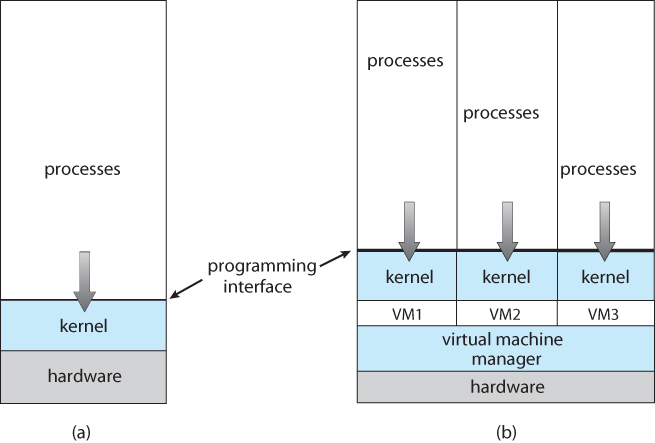
\includegraphics[width=10 cm, height= 8 cm]{virtuals.jpg}
\end{figure}
\end{center}

	
	
\textbf{ 3.3 Vulnerabilities, Threats & Risks}\\
	
	The cyberspace is challenged continually by vulnerabilities, threats and risks that have constantly spurred exploitation, conspiracy and conflicts. The increasing level of inter-dependence between physical and 
virtual components (technology), people and processes is relentlessly opening up unpredictable vulnerabilities,threats and risks. These span across software (viruses, worms, spyware, root kits, exploit scripts, protocol 
exploits, etc.), hardware (implantation of Trojans: undesired, malicious, deliberate alterations to electronic circuits) and human factor (insider or outsider threats, also from malicious or inadvertent actions or inaction in 
planning, design, implementation, deployment and operation). Thus, the notion of people in information systems is fundamental because systems are designed by humans, operated by humans and governed by humans; these key actions are subjective to human imperfection. The human factor, unescapably, cut across the life-cycle of providing and operating information systems infrastructure. For instance, when engineers design a system, it unavoidably often contains hardware flaws, software bugs or programming errors, meaning that since systems 
are products of human beings, mistakes are unavoidable. The consequence is that human error that is inevitably,persistently, can create security holes that may not be immediately perceived.There is no exploit (or threat) without vulnerability. Threats are continually evolving because of inherent vulnerability that is vary increasingly due to several factors. Simply, vulnerability is the state of visible weakness (exposure of weakness) that can possibly be exploited to carry out attacks or cause harm. Thus, a security breach is as a result of visible weakness found in a system. The unfortunate certainty, however, is that 
vulnerability in cyberspace infrastructure is likely to be eradicated, no matter the advances in cybersecurity controls. The dialectical relationship between threat, vulnerability and risk is that since, threat results from an 
exploitation of identified vulnerability in a system, risk is defined by the aftermath of the exploitation of any of such threat into a successful cyber-attack. The fact that criminality in the cyberspace is also creating innovations 
and opportunities within the cybersecurity industry is another paradox. It has become mice and cat race that no one is really sure who is obviously in the lead. The implication is that cybersecurity service providers are 
creating business opportunities from vulnerabilities. For instance, the production and sale of malware in one hand, and production and sale of anti-malware in the other hand in the past two decades, arguably, have
generated multibillion dollar businesses around the globe (ITU, 2008).
From the foregoing, it is evident that the interplay of cyber opportunities, negative or positive has strong elements of evolving vulnerabilities, threats and risks. What is clear in this context is that countries who aspire 
competitive lead in the vulnerability landscape and its exploitations can as well take undue advantage of others in the race for digital supremacy. Consequently, it can be argued that vulnerabilities, threats and risks are factors 
that are equally underpinning the undercurrents of the new world.\\

\textbf{ 3.4 Cyberwarfare }\\

	 Unlike in the last decade, cyber warfare is no longer strange or puzzling. With the emerging reality of state sponsored attacks on the cyber infrastructure of other nations, the entrenchment of the relatively new phenomenon of cyber warfare in human lexicon can hardly be contested. Cyber warfare from this perspective is an extension of the mutual web of conspiracy and sabotage between and among nations in conflict. In a cyberspace which is intrinsically challenged by uncertainties, State actors are ucnsatisfied with building defensive 
strategies alone but working effortlessly to build offensive capabilities that can assail their adversaries whenever desirable. Exacerbating this challenge is that no individual, organisation or government can provide an accurate 
profile of the threats and vulnerabilities evolving and emanating thereof. Consequently, it will appear that the raging war at cyberspace domain will be hard to win due to several factors that are too hard to predict. The 
factors that interplay and create the vulnerability landscape, which could be exploited by State actors against other States are inherently uncontrollable, arising, as more advancements are made in the technology arena. What 
has informed State actors is the same long tradition of worlds conspiracy and conflicts with taxonomy such as infiltration, sabotage, espionage, war, etc. as majority human activities shift to the new realm. As put by Ranger, 
(2015) after years on the defensive, governments are building their own offensive capabilities to deliver attacks It's all part of a secret, hidden arms race, where countries spend billions of dollars to create new armies 
and stockpiles of digital weapons.” What is key to all these exploits is the capability to latch onto the inherent vulnerabilities within the cyberspace through intensified and structured formal research and development –
searching for high profile vulnerabilities, which are hard to discover. That is, the strength of State actors lie in their skills and competence in discovering high-profile zero day vulnerabilities. The US, and other superior 
cyber-powers have already carved a career in this area with highly-profiled Vulnerability Researchers.The first attack, allegedly, arose international awareness, was the assault on Estonia, a Baltic State, with 
estimated population of about 1.3 million (BBC, 2007). Estonia, with claim of being the most internet-savvy State within the European Union, highly-dependent on cyber infrastructure, was seriously hit by sustained 
coordinated attack against government and critical private institutions websites causing heavy disruptions. This attack was remarkably an indication of potentially State backed conspiracy that could halt companies or even 
paralyse a State, as Russian State was suspected to have supported the attack (Ranger, 2015). Another publicly acknowledged cyberweapon or compromise masterminded by State actors i.e. Stuxnet, yet to be fully understood 
by military strategists, cyber security experts, and even political decision-makers in most countries, raised world attention (Bamford, 2013). Stuxnet, the cyberweapon that attacked the Iranian nuclear facility at Natanz is now 
the first acknowledged cyber incident within the scale and scope of cyber warfare. The mastery of the design and how it was able to undermine all security measures by the Iranians even against their computer networks that are 
isolated from the Internet network by a technology called air-gap continues to baffle cyber experts globally(Langner, 2013). Bamford, (2013), alleged that it was in 2012, anonymous source, revealed to The New York 
Times that America and Israel were responsible for the security breach in Iranian nuclear facility. The work that cumulated to Iranian attack, apparently, was a long years of US military‟s effort to develop offensive capabilities 
that is not only able to defend the US cyberspace but to equally batter its enemies Bamford, (2013). The Stuxnetcase, undoubtedly, demonstrated long period of professional and expertise development that attests to the undiscoverable nature of the weapon. There is an indication that the American National Security Agency (NSA) conceived “US Cyber Command” as far as the year 2000 to build US cyber warfare effort. According to Bamford, (2013), the US fears 
that cyberweapons are as crucial to 21st century warfare as nuclear arms were in the 20th. The US Cyber Command force is over 14, 000 personnel with over 13 formidable cyberattack teams declared Bamford, (2013).
The US sets aside 4.7 billion annually for developing cyberwarriors including high-profile expertise development, encouraging many doctoral degree studies in the various field of cyberspace (Bamford, 2013).
Conversely, the aftermath of Stuxnet incident was Iranian ferocious response. It was assumed that Iran hatched its counter on Saudi Aramco, an energy company and RasGas, the Qatari natural gas facility as well as 
several denial-of-service attack targeted on American interest (Perlrothoct, 2012). The Stuxnet sage also prompted Iran to form its Cyber Command, in attempt to building a tough Cyber force that is capable of 
inflicting damage to its foes (Langner, 2013).
In a similar development, China, alleged, has continuously invaded US cyberspace, increasingly,exploiting vulnerabilities in some military and government information systems and networks (Capaccio, 2012).
Capaccio, (2012), argued that most of the Chinese attacks are highly customised and specialized, with a high success rate targeted to vital military installations vulnerable to industrial espionage. Conversely, China assumed 
to be a deliberate contender of the US in the cyberspace, is building its cyber warfare paramilitaries, especiallyunderstood to be targeting US expertise and specialisations in communications, electronic warfare and 
networking skills. According to the US- China Economic and Security Review Commission, Chinas cyber capabilities is a worrying concern to the US, which fears that at any given point, China persistence, combined 
with notable advancements in exploitation activities pose growing challenges to information systems and their users (Capaccio, 2012). 
Similarly, the December, 2014 attack on Sony Pictures Entertainment, alleged committed by North Korea is another level of magnitude of attack that is capable of provoking cyberwarfare. The perpetuators of the 
Sony assault revealed embarrassing documents stolen from their exploits - private and personal sensitive information of employees of Sony amongst other critical data were compromised. The Sony attack raged public 
uproar in the US and US government was perturbed by the incident. North Korea, undoubtedly, is another strong contender and aggressor in the cyberspace with tracks of several coordinated attacks on South Korean interest. It 
has continued to assemble sophisticated cyber army for its offensive and defensive strategies. The UK, is not left in the cold, according to its Defence Secretary, Philip Hammond, we will build in Britain a cyber-strike 
capability so we can strike back in cyberspace against enemies who attack us, putting cyber alongside land, sea, air and space as a mainstream military activity" (Ranger, 2014).Debatably, these few examples and many others not highlighted here, are earlier warning that cyber 
conspiracy and conflicts capable of provoking a full scale conventional war or cyberwar or combination of the two, is no longer uncertain, however, the uncertainty, is when, and those who will be drawn to the cyber-battle 
fields. We argue that the widening global divide induced by the cyber revolution is yet to be recognised by most of the developing nations encumbered by several domestic problems and cultural issues. These local issues,
unavoidably, have continued to influence their poor perception of emerging trends. With the growing scale of conspiracy and conflicts, it is becoming increasingly critical that every nation State must strive to develop the capacity just as in the physical realm, to respond proportionately in the event of cyber conflict. This strengthens our argument, the need that part of the State requirement will be to develop the capability to deter the capacity of other States from conducting attacks against her interests
\begin{center}
\begin{figure}[h]
			\centering
			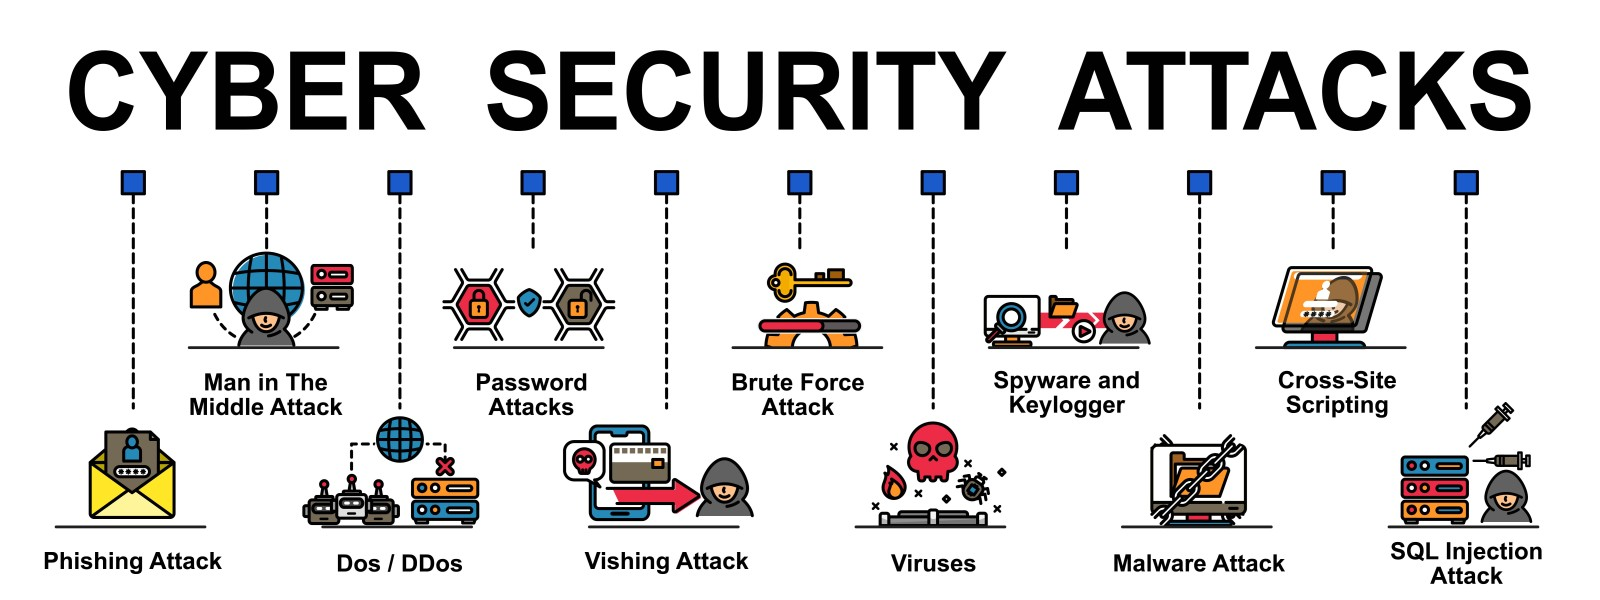
\includegraphics[width=12 cm , height=7 cm ]{cyberattack.jpeg}
\end{figure}
\end{center}






%---------------------------- End of Third Chapter------------------------------------
%---------------------------- Start of Last Chapter---------------------------------
\newpage
\begin{center}
\section{CONCLUSION}
{\setlength{\baselineskip}{1.5\baselineskip} }									
\end{center}

	Cyberspace is redefining a new world characterised by the ability of a State to compete advantageously with reasonable capacity and capability to excel in it. Countries are striving to have strong productive capacities in cyber products and  services, especially in  cybersecurity,  which is  a vital  component in  both  defence and offensive  strategies. The  real front-runners  are still  the developed  nations, and  the differentiator  in this  case remains the informed leadership issue. Our conclusion is that leaders of developed nations have  identified the criticality of  the new  world and are  in the  forefront of  its advancement  in all directions.  These leaders  have gained insight of the nuances of cyberspace and are convinced, so they have taken proactive steps to protect the
open cyberspace, defend it and bourgeon on it equally as they have with the physical world. For instance, the US, Britain, European countries, Russian, China, etc. through executive orders have extensive in-road and significant influence already on the cyberspace. They have shown leadership on the cyberspace by their actions – multiple strategies and initiatives in different facet of cyberspace domain that is setting the altitude for public and private sectors  evolvement. In  contrast,  absence of  political  maturity,  vague understanding of the new domain, and crowded domestic issues are responsible for slow adoption of strategies to harness the immense potentials of the cyberspace by developing nations. Sadly, as industrial revolution demarcated the world, so is the cyberspace fast bifurcating our global space


%---------------------------- End of Last Chapter----------------------------------------
%---------------------------- Start of Reference Chapter---------------------------------
\newpage
\begin{center}
\section{REFERENCES}
{\setlength{\baselineskip}{1.5\baselineskip} }									
\end{center}


List all the material used from various sources for making this project 
proposals 
\begin{enumerate}
\item Journal article - A. A. Author of article. "Title of article," 
Title of Journal, vol. \#, no. \#, pp. page number/s, Month year.

\item Books- Author's last name, first initial. (Publication 
date). Book title. Additional information. City of publication: 
Publishing company.

\item Magazine - Author's last name, first initial. (Publication 
date). Article title. Periodical title, volume number(issue number if 
available), inclusive pages

\item Website or Webpage Author's name. (Date of publication). Title 
of article. Title of Periodical, volume number, Retrieved month day, 
year, from full URL

\end{enumerate}

%---------------------------- Start of Reference Chapter---------------------------------

\end{document}
